\documentclass{article}
\usepackage[utf8]{inputenc}
\usepackage[a4paper, total={5in, 7.3in}]{geometry}
\usepackage{graphicx}
\usepackage{listings}

\lstset{basicstyle = \small}



\title{Security Analysis of Digital Post Application}
\author{Miłosz Głowaczewski}
\date{January 2024}

\begin{document}

    \maketitle
    \pagebreak
    \tableofcontents

    \chapter{Introduction}


\section{Garmin fitness watches}

In the past years fitness trackers experienced a high growth in popularity.
As the technology develops, the devices get more affordable and are able to track more metrics.
While it improves the insights into health and fitness tracking, it also means that it collects more sensitive data about the users.

Garmin fitness watches can accompany the users day and night, being able to last even over a week on a single charge.
The company has a wide range of options, having released over 100 different watches with third-party apps support\cite{garmin-connect-iq-devices}.
The devices are equipped with a large number of sensors such as heart rate, pulse oximeter, temperature, GPS, compass, accelerometer, gyroscope, altimeter, barometer, light sensor.
This allows collecting and calculating an enormous amount of different sensitive metrics.
As a result, the potential consequences of unauthorized access to the user's data are severe.

The watches can work independently, collecting and processing the data offline.
However, Garmin offers an extensive set of software to improve the user's experience.
There are multiple apps available for iPhone and Android phones to manage the watch and the data.
This means that the data is being sent over a Bluetooth protocol from the watch to the phone.
Additionally, Garmin encourages users to synchronize the data with their cloud.

In case the provided software does not fulfill users' requirements, it is also possible to install third-party apps on the watch.
Garmin maintains an ecosystem of tools for the developers to create apps and publish them in the Garmin store.
It makes the watch extensible and more universal, but it also allows for a third-party developer to gain access to some of the user data.

The described software offers a powerful toolset for the users to analyse their fitness data.
However, it also creates a large number of possible vectors of attack.
It is also important to notice that the Garmin software is not open source, which makes it more difficult to analyse its security.
Garmin provides a contact form on their website to report security vulnerabilities.
Unfortunately, they do not offer a bounty program.

In this report, a broad analysis of different attack vectors has been performed.

Overall, during the analysis, the following privacy and security concerns were found:
\begin{itemize}
    \item Garmin uses deprecated SHA-1 for watch third-party app signing
    \item Android apps installed on the phone, without any permissions can detect that the user uses Garmin devices and the type of the device
    \item Communication between the third-party apps and their companion apps are in plain text, available to all apps installed on the Android phone.
    I created a proof of concept app that can eavesdrop on the messages sent to the phone.
    \item Permission system of the third-party watch apps is not as well separated into different categories as it is in Android, iOS phones.
    \item Fuzzy testing suggests that it may be possible to escape the virtual machine running the third-party apps.
\end{itemize}


\section{Software description}
Garmin provides multiple mobile apps to manage the watch and the data.
\begin{itemize}
    \item Garmin Connect — the main app for managing the watch and the data.
    \item Garmin Explore — app for managing the watch and the data, focused on the offline usage.
    \item Garmin Connect IQ Store — app store for third-party apps, that can be installed on the watch.
\end{itemize}

If the user decides to synchronize the data with the cloud, it is sent to the Garmin Connect services.
Then it can be accessed through the website or the mobile app.

Additionally, Garmin has developed a proprietary programming language, Monkey C\footnote{\url{https://developer.garmin.com/connect-iq/monkey-c/}} running in a virtual machine for creating third-party apps.
The developers are provided with an SDK\footnote{\url{https://developer.garmin.com/connect-iq/overview/}}, containing all the necessary tools for creating and testing the apps.
Monkey C language has an integration with Visual Studio Code through the extension\footnote{\url{https://marketplace.visualstudio.com/items?itemName=garmin.monkey-c}}.
The apps can be tested either on a real device or on a simulator, provided with the SDK\@.
There is an official documentation describing the development process.

After a preliminary analysis, the following scripts and tools were found in the SDK:

\begin{itemize}
    \item monkeybrains.jar - java archive, compiles and builds the project
    \item simulator - binary ELF file, simulates a chosen Garmin device
    \item monkeydo - executes Connect IQ executable on the simulator
    \item Other scripts: barrelbuild, barreltest, connectiq, era, mdd, monkeyc, monkeygraph, monkeydoc, shell, monkeymotion
\end{itemize}

\section{Report structure}
The report structure roughly follows the order of the analysis.
Firstly, the threat model is described.
Then the security of the Garmin Connect IQ store is analysed.
With this knowledge, the security of the third-party apps is investigated.
This chapter describes the app runtime, building process and the communication between the watch and the phone.
After that, the fuzzing of the third-party apps is described.
At this stage, a custom fuzzer was created to test the security of the apps.
It generated promising results, opening additional opportunities for further research.

\section{Testing environment}
For the analysis the decision was made to use Linux operating systems as it is a popular choice in the system security community and a large number of materials use it.
The chosen distribution was Kali Linux because it comes with already preinstalled toolset.

The testing is executed on the watch Garmin Fenix 7S Pro, released in May 2023.
The third-party applications are investigated when using Connect IQ 6.3 SDK, released in August 2023.

Garmin supports both Android and iOS phones for managing the watch.
I focused on the Android version of the software.
Android is more open and easier to analyse, and I did not have access to Apple devices.


For the purpose of the analysis, when Garmin watches are mentioned, this report focuses on Garmin Fenix watches series 7.
Other devices may offer different hardware and software configurations.


\section{Related work}

Different attempts at the security analysis of Garmin software are available online.
There were attempts to ethically hack a Garmin watch\cite{kth-ethical-hacking,kth-audit}, analyzing different vectors of attack such as the Garmin Connect website, watch communication, and third-party apps.
However, they did not go deep into any of those topics.

Others tried to reverse engineer Garmin’s Virtual Machine and do a security analysis of the environment\cite{broken-vm,compromising-garmin-watches}.
They were able to get access to the firmware of the watch.
With the help of unofficial documentation of the firmware format\cite{firmware-format}, they proceeded to reverse engineer the bytecode.
During the analysis, they determined which parts of the code are responsible for the third-party apps' execution.
Thereafter, they found multiple vulnerabilities concerning the app runtime that have been disclosed to Garmin.
Some of them affected over a hundred devices for around 7 years.

While they explored the specific topic deeper, there is still a long list of things that could be analyzed in more detail.
Previous attempts used an available beta firmware for the analysis and used watches released over 4 years ago.
Since then, many new models have been introduced as well as new firmware versions with new features and expanded developer SDK.

Additionally, in 2020, Garmin was a victim of a ransomware attack\cite{garmin-ransomware-attack}.
The attack resulted in an inability to access several Garmin services for multiple days.

Considering the history of found vulnerabilities, the size of Garmin's ecosystem and the number of different components, the existing, publicly available analysis is far from being comprehensive.
    \section{Related work}

Different attempts at the security analysis of Garmin software are available online.
However, it is far from being extensive.
The amount of software, watch models and the fact that firmware is being constantly developed makes it infeasible to cover everything in a single publication.
There were attempts to ethically hack a Garmin watch[1][2], analyzing different vectors of attack such as the Garmin Connect website, watch communication, and third-party apps.
However, they did not go deep into any of those topics.
Others tried to reverse engineer Garmin’s Virtual Machine and firmware format[3][4][5].
While they explored the specific topic deeper, there is still a long list of things that could be explored.
Previous attempts used an available beta firmware for the analysis and used watches released over 4 years ago.
Since then, many new models have been introduced as well as new firmware versions with new features and expanded developer SDK.

    \section{Threat analysis}
\subsection{Focus of the analysis}
The amount of software, watch models, and the fact that firmware is being constantly developed makes it infeasible to cover everything in a single publication.
I decided to focus on the analysis of the third party apps, as it is the most interesting topic and unique to Garmin devices.
The previous research found multiple vulnerabilities in the third party apps runtime affecting over a hundred devices\cite{broken-vm,compromising-garmin-watches}.
Moreover, both of the articles mention that the analysis was far from being comprehensive.
Even though Garmin software is a closed source, the researchers were able to find multiple problems in the runtime environment.
This suggests it is worth investigating further, as there might be potentially more bugs in the software.

\subsection{Attack surface}
As the focus of the report is third party apps, the attack surface is limited to the apps and the store.
More precisely, for the attack surface, I will focus on the installation of malicious apps.
If the adversary is able to install a malicious app on the watch, it is possible to access sensitive user data and possibly tamper with it.
There are two stages of the apps that need to be considered:
\begin{itemize}
    \item Installation process
    \item Runtime
\end{itemize}

The watch is managed by the phone.
Because of that, for the security of the watch, it is important to consider the security of the phone as well.
Assuming that the phone itself is secure, the attack surface is limited to the Garmin mobile apps and the communication between the phone and the watch.
The installation of the apps is handled by the Connect IQ Store.
As such, the security of the store has to be analyzed.

The runtime is handled by the virtual machine, which is responsible for executing the bytecode of the apps.
Garmin provides a limited set of APIs that the apps can use.
When the user installs the app, they agree to the permissions requested by the app.
In this case, it is necessary to analyze if the apps can break the contract and access data or perform actions that they are not supposed to.
    \chapter{Security of Connect IQ store}
\section{Preliminary analysis}
\begin{figure}[h]
    \centering
    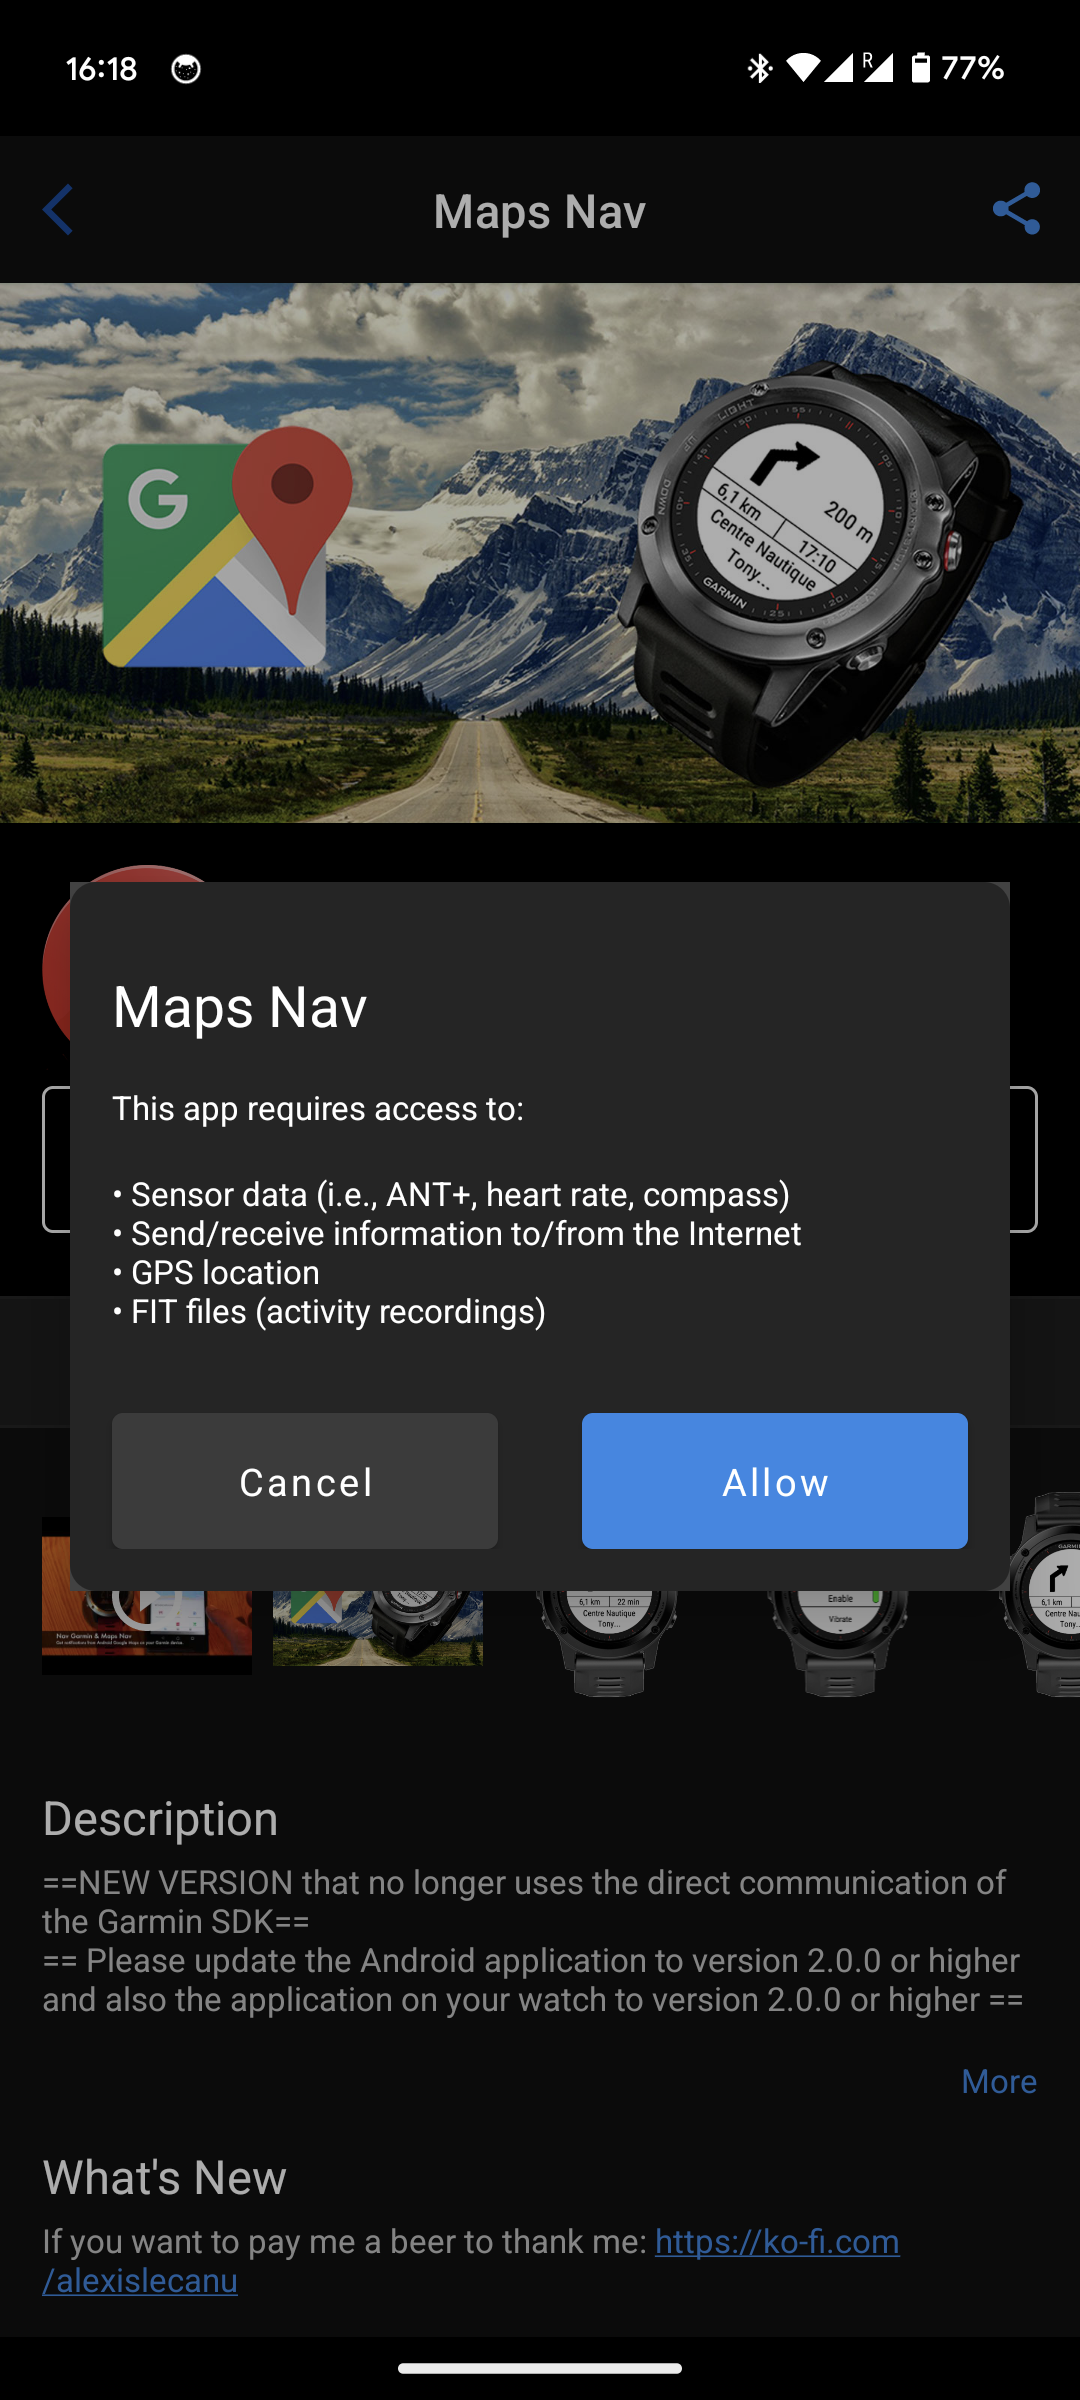
\includegraphics[width=0.3\linewidth]{../../images/connect-iq-app-permissions}
    \caption{Connect IQ - third-party app permissions request}
    \label{fig:connect-iq-store-permissions}
\end{figure}
Connect IQ store allows the users to browse and download third-party apps and watch faces to the watch.
The applications have descriptions and screenshots that can be added by the developers.
Additionally, users can write reviews and rate the apps.
Each app has information about the average rating and the number of downloads.
Before the app is downloaded, the user is presented with the information about permissions that the app requires, as presented in Figure~\ref{fig:connect-iq-store-permissions}.
The store also allows the users to create their own simple watch faces.

Based on the experiments with the watch, it seems that the app is downloaded to the phone and then sent to the watch via Bluetooth.

The analysis of the store does not go very deep, as I decided to focus more on the third-party apps.
However, it was necessary to have a basic understanding of the store, especially to analyze the communication between the watch and the phone.
This is described in the section~\ref{subsec:communication-watch-phone}.

\section{App decompilation}
\begin{figure}[h]
    \centering
    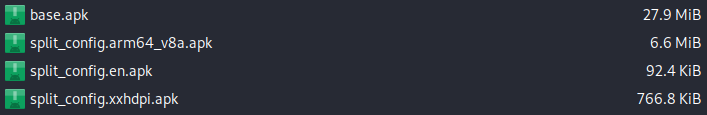
\includegraphics[width=0.7\linewidth]{../../images/connect-iq-apks}
    \caption{Connect IQ - Pulled apk files}
    \label{fig:connect-iq-apks}
\end{figure}
I installed the app on the phone and used $ADB$ to pull the apk files, that are presented in Figure~\ref{fig:connect-iq-apks}.
The app consists of multiple files, but the main one is \texttt{base.apk}.
It contains all JVM bytecode, which is the main focus of the analysis.
I decompiled the app with the JADX decompiler\footnote{\url{https://github.com/skylot/jadx}}.

The app is obfuscated.
It is a good practice as it makes the app size smaller and makes it more difficult to reverse engineer.
I was interested to find the code responsible for downloading the app to the phone and sending it to the watch.
Searching with several keywords, I was not able to find any code that would be responsible for checking the certificate of the downloaded app.
I was looking for names such as the library that was used to sign the app, SHA1, RSA\@.

Assuming that the watch is checking the certificate, it is not necessary for the phone to check it as well.
This is way it should be even safer, as the phone would be an additional attack surface.
With this conclusion, I decided to experiment later with the installation of an app that was not signed by the store in section~\ref{app-sideloading}.
%\section{Static analysis}
%
%Domain config is insecurely configured to permit clear text traffic to these domains in scope.
%
%It was detected that the is signed with MD5.
%MD5 hash algorithm is known to have collision issues.
%I couldnt verify it, to my knowledge the app was signed correctly.
%With signing scheme v2 and v3



\section{Sniffing the traffic}
To analyze the network security, I tried to sniff the traffic between the phone and Garmin servers.
I decided to use mitmproxy\footnote{\url{https://mitmproxy.org/}}.
When performing a dynamic analysis, there are two options.
Either use an emulator or a real device.
Emulator usually offers more flexibility and is easier to manipulate.
However, it does not have access to Bluetooth, which is necessary to test the Connect IQ store.
For this reason, I used a real device.

\begin{figure}[h]
    \centering
    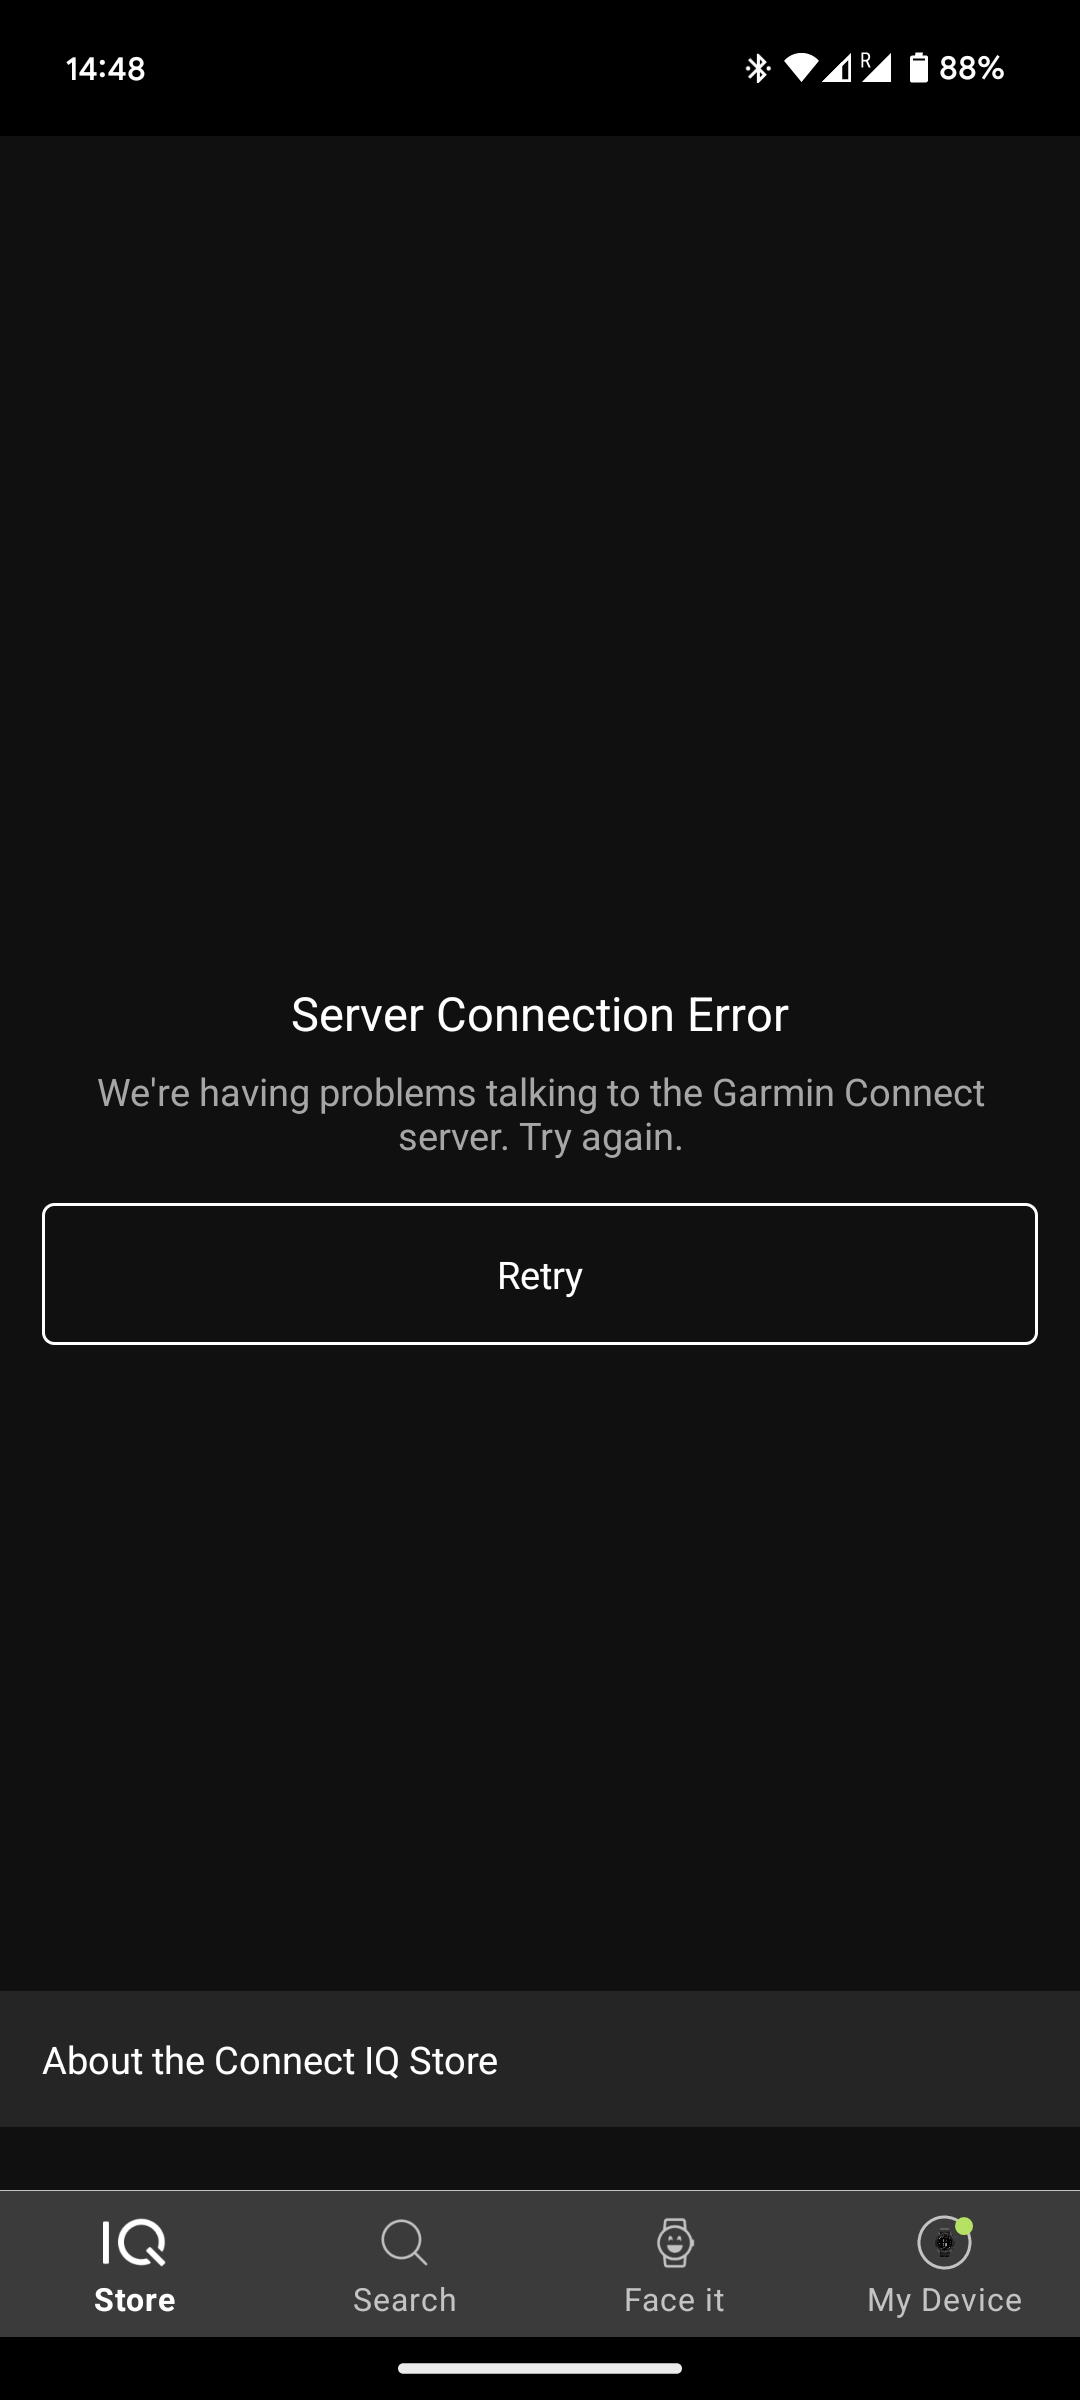
\includegraphics[width=0.3\linewidth]{../../images/connect-iq-connection-failed}
    \caption{Connect IQ refusing to connect}
    \label{fig:connect-iq-connection-failed}
\end{figure}

I configured the computer to act as a hotspot, started mitmproxy and forwarded the traffic there.
Then I connected the phone to the hotspot, and I was able to capture the traffic.
However, when connecting to the mitmproxy, the app refused to connect, as presented in Figure~\ref{fig:connect-iq-connection-failed}.
This means that the app is checking the certificate of the server and man-in-the-middle attack is not easy to execute.
After adding the mitmproxy certificate to the phone, the app would still refuse to connect.
The app is probably using a default Android certificate configuration, which does not trust user added certificates.
This is the case for all recent Android versions.
As the minimum supported version by Connect IQ is Android 7, it would be required to have root access to add certificates accepted by applications.
Another option is to modify the app to accept user added certificates.

\subsection*{Attempt 1 — Android Unpinner}
I tried to use Android Unpinner\footnote{\url{https://github.com/mitmproxy/android-unpinner}}.
It is an open-source tool that modifies the app to remove certificate pinning.
After installing the modified app, it was possible to sniff the traffic.
However, it was not possible to log in.
When trying to do so, it would go back to the welcome screen every time.

\subsection*{Attempt 2 — manually modify the apk and sign again}

I decided to try to modify the app manually.
I used Apktool\footnote{\url{https://apktool.org/}} to unpack the app.
Then I modified the network security configuration file to accept the user added certificates.
After that, I packed it again, aligned zip file and signed with a debug key.
After installing the app, there were some errors with missing resources.
I did not investigate it further.

\subsection*{Attempt 3 — only resign the app.}

To check if there is any potential in this approach, I decided to try to resign the app without any modifications and any proxy.
The app started, but again it was not possible to log in, it would go back to the welcome screen as in the first attempt.
I was not able to find what was the reason for that.
I could not find anything in the request logs from mitmproxy.
Sometimes hash of the fingerprint is used to identify the app by some services.
However, I did not find any evidence of that.

\subsection*{Attempt 4 — use rooted phone}
After the previous failed attempts, I decided to try to use a rooted phone.
I used my old, no longer used phone — Samsung S20.
To root the phone, I followed the instructions found on the XDA Forums\footnote{\url{https://xdaforums.com/t/how-to-exynos-snapdragon-root-s20-series-and-upgrade-firmware.4079353/}}.
Then I was able to install the mitmproxy certificate as the system certificate and use the original app.

\section{Network security}
Finally, I was able to sniff the traffic, as presented in Figure~\ref{fig:mitmproxy-unpinner}.
Based on the traffic that went through mitmproxy, I was able to determine Garmin domains used by the app.
I used Qualys SSl Labs\footnote{\url{https://www.ssllabs.com/ssltest/}} to analyze their security.

\begin{itemize}
    \item \textit{sso.garmin.com} - Received grade B because the server still supports TLS 1.1.
    It is not optimal, as there are known vulnerabilities of this protocol.
    \item \textit{diauth.garmin.com} - Received grade A, analysis did not find any issues.
\end{itemize}

\begin{figure}[h]
    \centering
    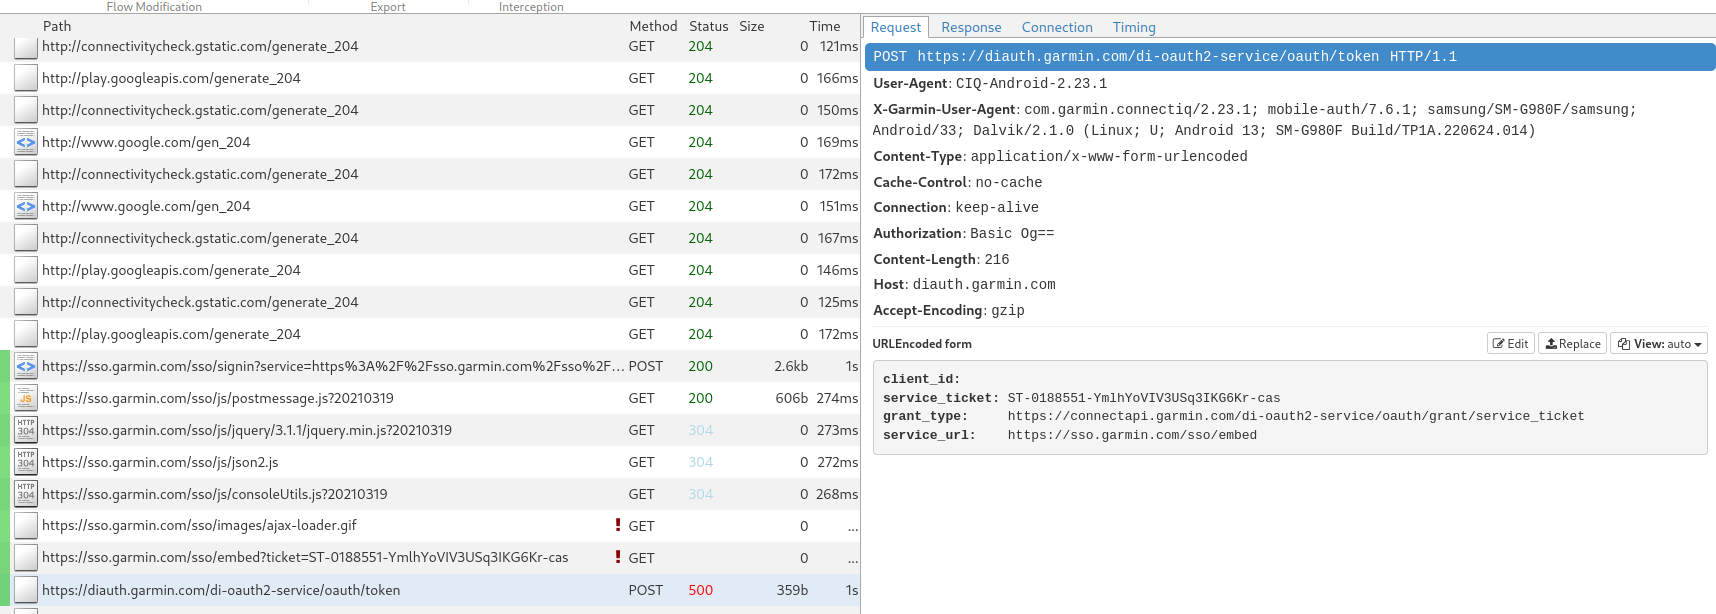
\includegraphics[width=1\linewidth]{../../images/mitmproxy unpinner}
    \caption{Sniffed traffic}
    \label{fig:mitmproxy-unpinner}
\end{figure}

Additionally, as the app allows the users to add their content, I looked at how it is handled.
The developer creates a description of their app, screenshots, and other information.
Moreover, other users can comment on the app.
With this type of content, it is important to be aware of potential attacks if the text is not parsed correctly.
Fortunately, in the case of native Android apps, usually attacks known from web applications are not possible.
Nonetheless, if the text is not parsed correctly, it could be a potential vector of attack.
However, it seems that everything is sent as a plain text.
It looks like there are no tags or any special parsing.
In this case, it should not be possible to perform any attacks based on improper sanitization of the input.
%\section{Communication between the watch and the phone}
%I considered analyzing the communication between the watch and the phone.
%However, it uses Bluetooth LE Secure Connections.

\section{App sideloading}
\label{app-sideloading}
Garmin allows the developers to install the app on the watch through the cable.
I was interested to see if it is possible to install an app not signed by the store remotely.
I tested it by replacing the app that would be downloaded from the store with the one that I created.
When the app is installed, the phone downloads the app from the store and sends it to the watch.
With the help of the mitmproxy, I was able to capture the request and replace the app with a different one.
After experimenting with different apps, the watch would refuse to install any app not signed by the store.
It was possible, however, to replace the app with another one, signed by the store.
This means that the watch is probably checking the certificate of the app.

It suggests that the API for remote app installation requires the app to be signed by the store.
This is a good thing, as it helps to prevent the installation of malicious apps.

    
\chapter{Security of third-party apps}

\section{App runtime}

The applications are intended to be run on a wide range of devices, with different hardware configurations.
The execution environment needs to be able to enforce access control and isolation.
Moreover, the devices are very limited in resources, which makes it difficult to adapt the existing solutions such as Java virtual machine.
For those reasons, Garmin decided to create a custom virtual machine and a programming language.

However, creating a correct abstraction layer is a complex task.
It creates a large attack surface, and it is challenging to ensure that the implementation is correct.

\section{Preliminary analysis}
The existing research analysed the bytecode of the firmware running on the watch.
Unfortunately, the firmware is no longer available for download.
There is a chance that it would be possible to reverse engineer the watch hardware and extract the firmware from the device.
However, it would require an extensive amount of time and resources and is out of scope of this report.
Another option would be to investigate the protocol used to download a new firmware version.
It would require additional time and there is no guarantee that it would be possible to download the full firmware.

In the end, I decided to perform the analysis on the simulator provided by Garmin.
As it runs directly on the computer, it is possible to perform a more in-depth analysis of the software such as dynamic analysis.
The simulator is supposed to guarantee proper isolation, so escaping the sandbox could be a potential vulnerability being a threat to the computer.
Additionally, there is a chance that parts of the code are reused in the firmware running on the watch and the findings would be applicable to the real device.

\section{Permissions}
\begin{figure}[h]
    \centering
    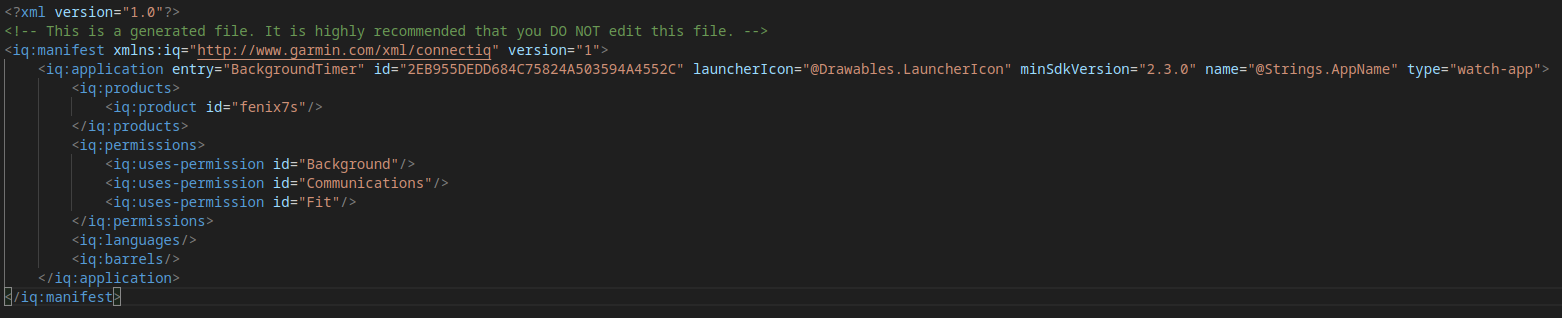
\includegraphics[width=1\linewidth]{../../images/garmin-app-manifest}
    \caption{Garmin third-party app manifest}
    \label{fig:garmin-app-manifest}
\end{figure}
Third-party apps can interact with the watch by using the API provided by the SDK.
The API is divided into several modules, each of them providing different functionality.
Some of those functionalities can be considered sensitive, such as GPS location, heart rate, or access to the internet.
Because of that, Garmin implemented a permission system, where different permissions grant access to different modules.
The app has to define in the manifest file which permissions it requires, and the user has to accept them before installing the app.
The manifest file is presented in the figure~\ref{fig:garmin-app-manifest}.
The system offers some granularity, and can give the user a general overview of what the app can do.
However, some, potentially sensitive modules don't require any permissions.
For example, the app can access some basic activity data such as heart rate, steps, calories without any permissions.
Moreover, in February 2023, Garmin introduced a new module: Complications.
It is a publish/subscribe model that allows for the apps to publish different metrics, so that they would be accessible for any watch face.
While it makes the access to different metrics more flexible and accessible, it also removes the granularity of the permissions.
Every app can potentially publish very sensitive data, without the user being aware of it.
Then every watch face can access all this data if it requests \textit{Complications} permission.

\section{Building process}
In order to understand the runtime environment, I started with the analysis of the building process.
As it was mentioned, it is recommended to use Visual Studio Code with the extension provided by Garmin.
The program is written in Monkey C language.
For testing purposes, the app can be run on a simulator or a real device.
The extension provides a user interface to automatically install the app on the simulator.
It is also possible to generate a binary PRG file that can be installed on the watch.
Before the app can be installed on the watch, it has to be signed by the developer.

During the compilation, the code is translated to mid-level intermediate representation (MIR).
The files containing the representations could be used for better understanding of the final artefact.

Visual Studio calls the compiler, which is a jar file called \textit{monkeybrains.jar}.
The compiler is written in Java, which makes the analysis of the code relatively straightforward.
Nonetheless, it is a complicated process consisting of several stages.
For the analysis, I decided to use the JADX decompiler\footnote{\url{https://github.com/skylot/jadx}}.

After loading the jar file, I noticed that a large part of the relevant code is not obfuscated.
Then I proceeded to analyse the code.
The following classes are of particular interest:
\begin{itemize}
    \item \texttt{com.garmin.monkeybrains.compiler2.Compiler2} — main class responsible for the compilation process.
    \item \texttt{com.garmin.connectiq.common.monkeyc.AssemblerOpcode} — contains a list of instructions in the final bytecode.
    \item \texttt{com.garmin.connectiq.common.signing.SigningUtils} — class responsible for signing the app, described in more detail in the section~\ref{subsec:signing}.
\end{itemize}
Additionally, the SDK provides a mapping of all API methods to the number values.
This is probably used by the virtual machine to identify the method that should be called.

I was able to find the code responsible for signing the application.
It is described in more detail in the section~\ref{subsec:signing}.

\section{Signing} \label{subsec:signing}
Garmin requires that the apps are signed to be installed on the watch\cite{garmin-signing}.
The app has to be signed by the developer with their private key.
In order for the app to be updated, it has to be signed with the same key.
When the store has approved the app, it is additionally signed with the store signature.

The described process enforces that the app can be updated only by the developer having access to the original private key.
Additionally, when the app is downloaded from the store, the watch can verify that it has been approved by the store.

Based on the analysis of the compiler, class \texttt{SigningUtils} is responsible for signing the app.
It uses \texttt{java.security.Signature} class to generate the signature.
The signing algorithm uses SHA1 hash of the bytecode that is signed with a private RSA key.
The key is 4096 long, which is more than recommended.
For the signing, conventions described in PKCS \#1 v2.2 are used\cite{java-signature,pkcs}.
The pseudocode of the signing algorithm is presented in the listing~\ref{lst:signing}.
The signature computed by the store is generated in a similar way, does not include the modulus and exponent, and uses a different magic number.
The store probably uses the public key in the developer signature to verify and save it after the first upload of the app.
\begin{lstlisting}[caption={Pseudocode of the signing algorithm, developer signature},captionpos=b,label={lst:signing},language=Python]
    def sign_with_developer_signature():
        app_bytes = read_prg_file()
        app_bytes, terminator = remove_terminator(app_bytes)
        signature, modulus, exponent = compute_signature(app_bytes)

        dev_signature = byte_array()
        dev_signature.append(magic_number)
        dev_signature.append(signature_length)
        dev_signature.append(signature)
        dev_signature.append(modulus)
        dev_signature.append(exponent)

        signed_app = byte_array()
        signed_app.append_all(app_bytes, dev_signature, terminator)
        write_prg_file(signed_app)
\end{lstlisting}

SHA-1 is no longer considered secure against well-funded opponents.
NIST formally deprecated use of this hash function in 2011.
In 2020 there was a paper published demonstrating a chosen-prefix collision attack.
A potential vector of attack would be to create a malicious app with the same hash as the original app.
At the current state of the art, there is no viable solution to find a collision to a given hash for a chosen prefix.
However, the function has been already broken and in the upcoming years new attacks might be discovered.

\section{Modifying the executable}
\label{sec:modifying-the-executable}
To perform dynamic analysis of the virtual machine, it is useful to be able to edit the executable.
However, after changing the bytecode, it is necessary to sign the executable again.
With the knowledge gained from the previous section, I created a Kotlin script that signs the app again.

The code follows the same instructions as the original method in listing~\ref{lst:signing}.
The only difference is that the old signature is replaced with the new one.

\begin{figure}[h]
    \centering
    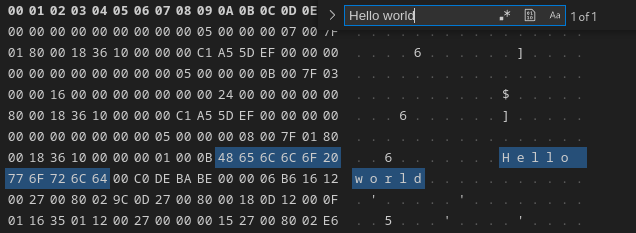
\includegraphics[width=0.7\linewidth]{../../images/app-hex-editor-hello-world}
    \caption{Prg file in hex editor}
    \label{fig:hello-world}
\end{figure}

To verify that the script works correctly, I created a simple app that shows a message 'Hello world'.
Then I opened the PRG file in a hex editor and searched for the message, as presented in the figure~\ref{fig:hello-world}.
Consequently, I modified the string and signed the app with the created script.
After installing the app on the watch and the simulator, the new message was displayed.
When trying to install the app without the new signature, the watch and the simulator would display an error message.

\section{Simulator}
Garmin SDK provides a simulator for testing the apps.
It is used by the Visual Studio Code extension to run the apps.
I found the executable in the SDK bin folder.
The file starts with ELF header, which means that it is a binary executable file.
To analyse bytecode, I decided to use Ghidra\footnote{\url{https://ghidra-sre.org/}}.
It is free and open-source software for reverse engineering.

After loading the file, a list of assembly instructions is displayed.
Fortunately, Ghidra has an option to analyse and decompile the code to C\@.

\begin{figure}[h]
    \centering
    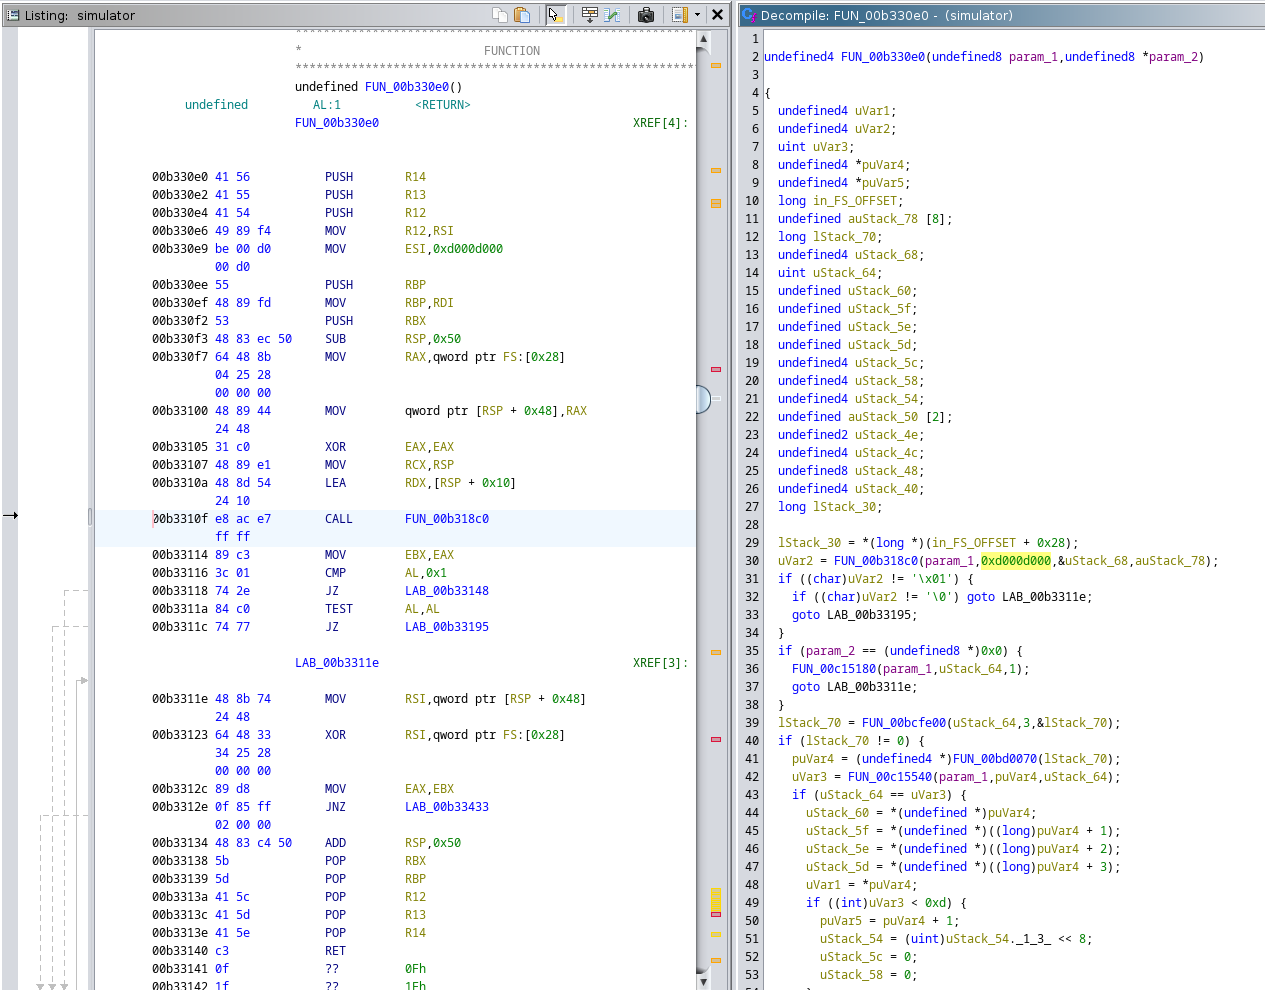
\includegraphics[width=0.7\linewidth]{../../images/ghidra}
    \caption{Simulator decompilation}
    \label{fig:concept}
\end{figure}

The header of the third-party apps is tagged with value `0xD000D000`\cite{broken-vm}.
Searching for it in the simulator binary reveals two references.

From this point, it would be theoretically possible to analyse the code and reverse engineer the virtual machine.
However, doing it without any documentation, where the names of the functions and variables are not known would be very challenging.
As it is not possible to do it in a reasonable amount of time, I decided to focus on fuzzing the virtual machine.
This is described in the section~\ref{sec:fuzzing}.

\section{Communication between the watch and the phone} \label{subsec:communication-watch-phone}

Garmin has multiple apps for managing the watch and the data.
As such, it is interesting to analyse the communication between them and the watch.
I analyzed the Manifest files in Connect IQ Store and Garmin Connect apps.
Both of them use Bluetooth permissions to connect with the watch.
Additionally, they define Garmin custom permissions as can be seen in the figure~\ref{fig:connect-iq-declared-permissions}.
The permissions have set protection level to `signature`(0x2), which means that only apps signed with the same key can use them.
They are used to be able to receive specific broadcasts, probably to communicate with themselves.
It is a functionality provided by Android and should offer an appropriate level of security.

\begin{figure}[h]
    \centering
    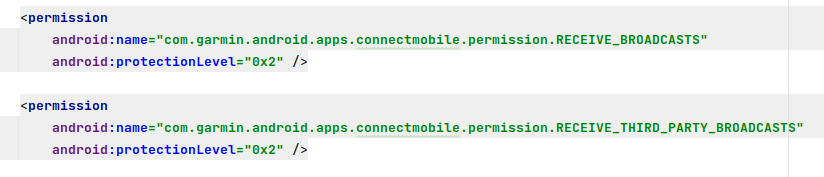
\includegraphics[width=1\linewidth]{../../images/android-declared-permissions}
    \caption{Declared permissions by Connect IQ Store}
    \label{fig:connect-iq-declared-permissions}
\end{figure}

When it comes to third-party apps, they can communicate with the phone by using the API provided by the SDK\@.
Garmin created SDK for Android and iOS that allows to create a companion mobile app for the watch app.
They created an example of watch and Android app that communicate with each other\footnote{\url{https://github.com/garmin/connectiq-android-sdk}}.
The Android SDK uses Broadcasts under the hood to communicate with Garmin Connect app.
The SDK allows the programmer to query for available Garmin devices connected to the phone.
Then it is possible to establish communication with a chosen app on the watch.

The first thing that can be noticed is that the SDK is able to get a list of all Garmin devices connected to the phone without any permissions.
They use Broadcasts that are available to all apps.
This creates a potential privacy issue, as any app can get the information if the user has a Garmin device connected to the phone.
Moreover, it is possible to get the information about the device, such as the model name.

Another issue is that the communication between the app on the watch and the companion app is not protected or encrypted.
The SDK offers a function to register a listener for events from the watch app, given the app ID\@.
However, when looking at the implementation, it is a wrapper around the Broadcasts.
It is possible to register a listener for all events from all apps.
This means that any app on the phone can listen to the messages from any watch app.
I did not find any mention that would warn the developers about this fact.

Following this finding, I decided to test this hypothesis.
I created a simple watch app that sends a message to the companion app.
Then, based on the SDK, I created an Android app that listens to all messages from all watch apps.
When I installed both apps, the Android app was able to receive the messages from the watch app with the information about the origin.

Having this information, I proceeded to investigate if it might be an issue for existing apps in the store.
Firstly, I looked into Spotify and Komoot apps.
Both of them are very popular and have a large number of downloads.
They have a full version of the app available on the phone and a companion app on the watch.
However, they do not use the mobile SDK provided by Garmin.
Instead, they connect to their servers directly.
It might be because it was easier to implement, or because they wanted to have more control over the communication.

Then I tried to find apps that use the mobile SDK provided by Garmin.
I found a developer 'r.485' that has published multiple apps in the store with the companion app on the phone.
However, when I installed the apps, they did not work correctly.

At this point, I decided to stop the investigation.
While it is a privacy issue, I could not find any apps that it would affect.


As Garmin already uses custom permissions for communication between their apps, I wondered why they did not use it for the SDK\@.
According to Android documentation,\cite{android-broadcasts} it is possible to send broadcasts that can be only received by apps with specific permissions.
It is also possible to define a custom permission that can be requested by other apps.
However, custom permissions have to be already defined when such an app is being installed.
This is not always the case, and because of that, it is probably not a viable option for Garmin.

    \chapter{Fuzzing third-party apps} \label{sec:fuzzing}
\section{Introduction}
Static analysis of assembly code is a very time-consuming process that requires extensive knowledge.
Without any documentation, source code provided by the vendor, or any other help, it is extremely difficult to understand the code.

For this reason, I decided to use dynamic analysis to find vulnerabilities in the code.
As I am focusing on analysis of the virtual machine in the simulator, there are more possibilities to test the behaviour during runtime.
The simulator allows running the code in a controlled environment, which makes it easier to test different scenarios.
With this approach, there is no need to understand the code.
It is also valuable when the code base is large and complex.
Additionally, instead of spending time on reverse engineering, it is possible to write a fuzzer that will do the difficult work.
Sometimes it might be necessary to run the fuzzer for a long time.
This, however, does not require any human interaction and can be scaled to run on multiple machines or threads.
The expected outcome of the fuzzer is a binary file that crashes the virtual machine and can be run on the watch.

Finding vulnerabilities in the simulator is aimed at achieving two potential objectives.
Firstly, it might be possible to escape the sandbox and for example, execute arbitrary code on the host machine.
Secondly, vulnerabilities in the simulator might be present in the real device as well.

\section{Environment setup}
When fuzzing a program, the most basic configuration would be to have a fuzzer and provide it with a program and the starting input.
Then the fuzzer would run the program with different modifications of the input and check if it crashes.

However, in this case, the setup is more complicated.
Simulator is run as a standalone program.
Then the application has to be loaded with an additional command line script.
As such, the fuzzer needs to be aware of both tools.

Moreover, when modifying the input, the virtual machine requires it to be signed.
This means that to test the execution after each modification, the input needs to be signed again.


\section{Fuzzing solutions}
One of the most popular fuzzing solutions is AFL++\cite{aflplusplus}.
It is an improved fork to Google's AFL\footnote{\url{https://github.com/google/AFL}}, which is no longer maintained.
AFL++ is an open-source tool for fuzzing a wide range of software.
It is coupled with instrumentation-guided genetic algorithm, having a possibility to be extended for different use cases.

AFL++ is a very powerful tool when the source code is available.
This allows it to be compiled with a special compiler that adds instrumentation to the code.
This way the fuzzer can monitor how the changes in the input affect the execution of the program, increasing the amount of code coverage.

However, in this case, the source code is not available.
One option would be to run it without instrumentation.
Another one would be to execute the simulator in a processor emulator, such as QEMU\footnote{\url{https://www.qemu.org/}}.
It would also be necessary to write a custom mutator that would modify the input and sign it again.
Additionally, there are two programs that need to be run: the simulator and the script that loads the application.
It would require some additional configuration to make it work with AFL++.

With those factors in mind, I decided to write a custom fuzzer that would be tailored to the needs of this project.
This way, it would be easier to debug and modify the fuzzer to fit the requirements.
Additionally, it would be a valuable learning experience to write it from scratch.


\section{Fuzzing process}
\begin{figure}[h]
    \centering
    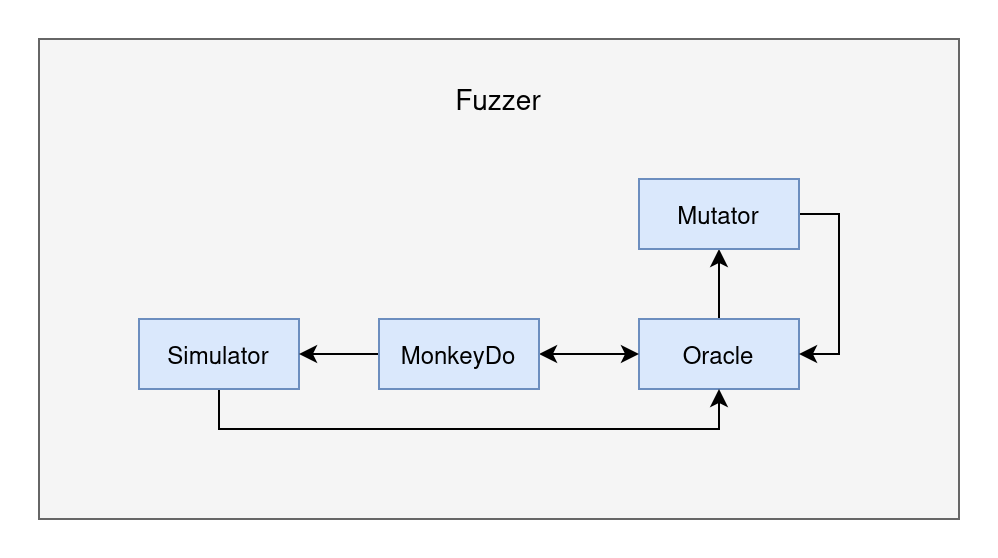
\includegraphics[width=0.8\linewidth]{../../images/fuzzer-diagram}
    \caption{Fuzzing process}
    \label{fig:fuzzer-diagram}
\end{figure}

The fuzzer consists of four main components: Mutator, Simulator, MonkeyDo, and Oracle, as presented in Figure~\ref{fig:fuzzer-diagram}.
The fuzzing is performed in an iterative manner.
The Mutator generates a new input, then Oracle tests the execution of the input.
Based on the result, the Mutator either mutates the current input or reverts the previous mutation.
This way, the input oscillates closely between two states: one that barely works and another one that does not run successfully.
With this continuous modification of the input, the fuzzer explores different variations of the bytecode until it finds one that is not handled correctly by the virtual machine.
To make it possible to reproduce the steps, the fuzzer uses a random generator with a fixed seed, defined at the beginning of the script.


\subsection*{Mutator}
\begin{lstlisting}[caption={Pseudocode of the mutating algorithm},captionpos=b,label={lst:mutator},language=Python]
originalApp = load("seed_app.prg")
currentApp = originalApp
lastMutation = emptyList()

def mutate(passed: Boolean):
    if passed:
        mutateCurrentApp()
    else:
        revertMutations()
    return sign(currentApp)

def mutateCurrentApp():
    mutation = generateMutation()
    for byte in mutation:
        currentApp[byte] = flipRandomBit(currentApp[byte])
    lastMutation = mutation

def revertMutations():
    lastMutation, bytesToRevert = splitInHalf(lastMutation)
    for byte in bytesToRevert:
        currentApp[byte] = originalApp[byte]

def generateMutation():
    mutationSize = mutationRate*len(currentApp)
    return [randomByte() for i in range(0, mutationSize)]
\end{lstlisting}

Mutator is responsible for generating a new input for the simulator.
It does that by mutating the original(seed) application and signing it again as described in section~\ref{sec:modifying-the-executable}.
The pseudocode of the mutating algorithm is presented in Listing~\ref{lst:mutator}.
Depending on the result of the previous execution, the mutator either mutates the current application or reverts the previous mutation.
To make the process more efficient, the mutator does not revert the whole mutation, but only half of it.
Using the divide-and-conquer approach, it is possible to find the byte that broke the application faster.


\subsection*{Simulator}
%\begin{figure}
%    \centering
    \begin{figure}[b]
        \centering
        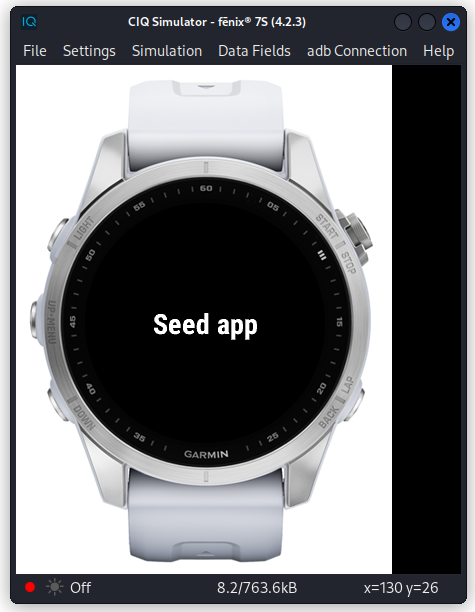
\includegraphics[width=0.39\linewidth]{../../images/simulator-seed-app}
        \caption{Simulator running seed app}
        \label{fig:simulator-seed-app}
    \end{figure}
    \begin{figure}
        \centering
        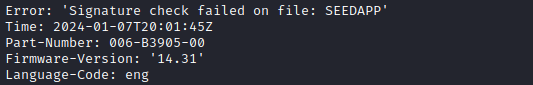
\includegraphics[width=0.6\linewidth]{../../images/simulator-signature-failed}
        \caption{Simulator output when signature verification fails}
        \label{fig:simulator-signature-failed}
    \end{figure}
%    \caption{Simulator}
%\end{figure}
The simulator component is responsible for running the simulator executable.
In Figure~\ref{fig:simulator-seed-app}, the simulator is running the seed application.
The component monitors the output of the simulator, which can be used by the Oracle to decide if provided input has been executed successfully.
This information is needed to decide if the mutator should mutate the current application or revert the previous mutation.
Example output of the simulator is presented in Figure~\ref{fig:simulator-signature-failed}.
Additionally, the component detects when the simulator crashes.
This information is used by the Oracle component to determine if a bug has been found.

\subsection*{MonkeyDo}
Oracle component is using MonkeyDo script to load the application into the simulator.
The script outputs logs from the loaded application.
It also does a partial parsing of the application and might sometimes output errors.


\subsection*{Oracle}
The Oracle component tests the execution of the application generated by the Mutator.
It uses the output of the Simulator and MonkeyDo to determine if the execution was successful.
At this stage, it was important to investigate possible outputs of the MonkeyDo script and the simulator.
Based on those outputs, a decision is made if the application should be mutated or reverted.

The app is programmed to print a message \textit{Okay} when it is executed.
This message is used to determine if the execution was successful.
However, it may take a few seconds for the message to appear.
To speed up the process, the Oracle also checks if any of the expected error messages has been printed.
If this is the case, the execution is considered to be unsuccessful.

Sometimes when the application is modified, the simulator will output an error message that signature check failed.
The message contains the name of the app file.
When this happens, the application is considered invalid and the mutation is reverted.
However, sometimes the same output is produced again when the next application is loaded.
Because of that, every version of the application has to have a different file name.
This way, it can be determined if the error is caused by the previous application or the current one.


\section{Fuzzing results}

For the fuzzing, I created a simple application that prints a message \textit{Okay} when executed.
The application is based on an example provided by the SDK, called \textit{Confirmation Dialog}.

I was running the fuzzer with at most 50 iterations, so that it would be possible to easily reproduce all steps.
Each run of the fuzzer started with a different seed for a random generator.
The Oracle was configured to timeout after 15 seconds if the application did not print the expected message.

After the first run, I noticed that sometimes there would be an error message: \textit{Permissions required}.
Probably some modifications caused the application to access parts of the SDK that it did not have permission to.
After this finding, I decided to modify the application to request all permissions.
This way, it would be possible to detect potential bugs in all parts of the SDK\@.

\begin{figure}[h]
    \centering
    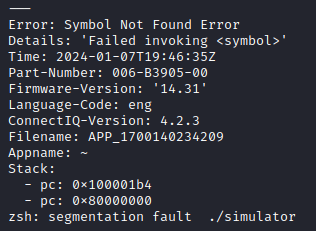
\includegraphics[width=0.4\linewidth]{../../images/simulator-crash}
    \caption{Simulator crash}
    \label{fig:simulator-crash}
\end{figure}

With this configuration, the fuzzer was able to consistently find an input that was crashing the simulator.
Roughly every second or third run of the fuzzer a new such input was found.
The crash was caused by a segmentation fault error, as presented in Figure~\ref{fig:simulator-crash}.
This is a bug in the simulator, as it should not crash when executing an application.
However, it is challenging to assess if this bug can be exploited.
Potentially, it might be possible to escape the virtual machine and attack the host machine.
However, it would require a further investigation into the machine code of the simulator.

\begin{figure}[h]
    \centering
    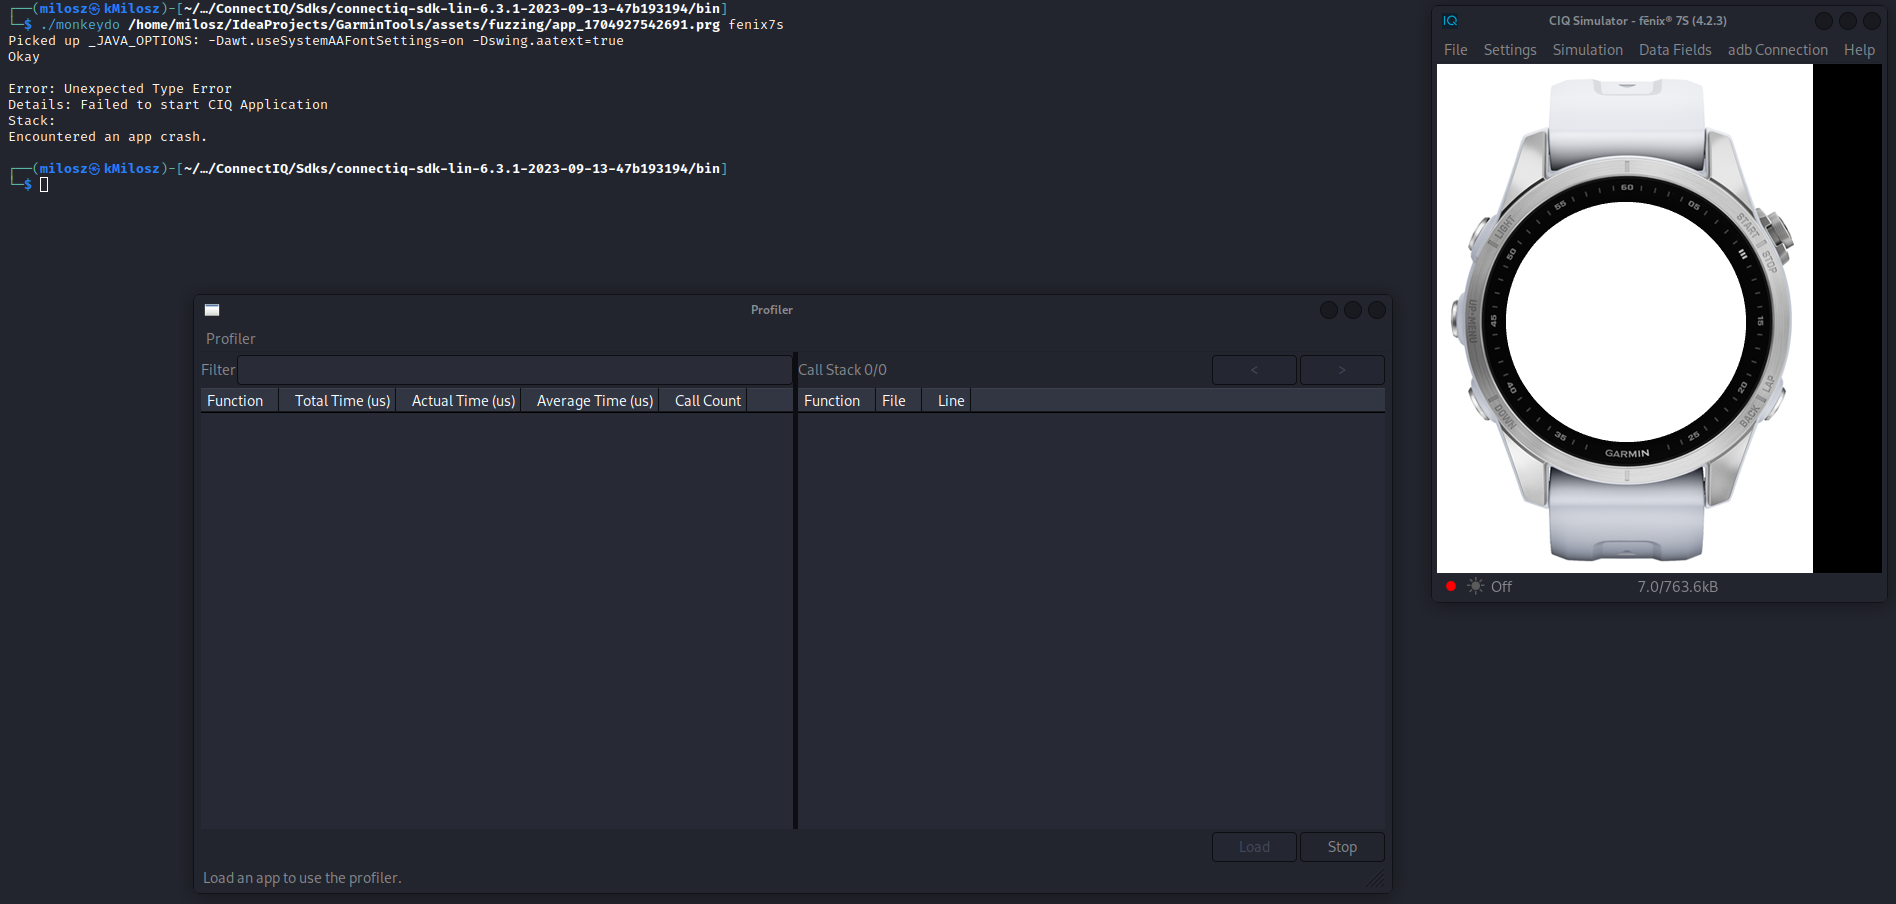
\includegraphics[width=1\linewidth]{../../images/simulator-bug-profiler}
    \caption{Simulator starting the profiler}
    \label{fig:simulator-bug-profiler}
\end{figure}

Additionally, I tried to fuzz the application without any permissions to compare the results.
It seemed that the crashes were happening more rarely.
However, during one of the runs, I noticed a strange behaviour of the simulator.
Once, when the application was executed, the simulator started profiling and opened a window with the profiler, as presented in Figure~\ref{fig:simulator-bug-profiler}.
The application was executed, printed the message \textit{Okay}, and then crashed.

In the beginning, I thought that it might be a bug in the simulator.
Trying to find an explanation for this behaviour, I looked into the documentation of the simulator.
After some investigation, I found out that there is a compiler flag that enables the profiler during the execution of the application.
Probably, the mutation caused the flag to be enabled.

Having multiple applications generated by the fuzzer, I experimented with loading them into a real device.
The applications were successfully installed on the watch.
Unfortunately, I did not observe any unexpected behavior and the watch did not provide any additional logs.
Based on this, it is not possible to assess if the bug is present in the real device as well.
It would require further investigation into the watch.

Those results show that there are bugs in the simulator, potentially also affecting real devices.
Even though the fuzzer did not use instrumentation, it was able to consistently find an input that crashes the simulator in under 15 minutes.
It suggests that there might be multiple bugs in the simulator and virtual machine.
This opens an opportunity to continue the investigation to assess if it is possible to find any vulnerabilities that can be exploited.
    \chapter{Privacy}

    \chapter{Conclusion}
\section{Summary}

The goal of the project was to analyze the security of the Garmin watches and the third-party apps.
During the analysis, the ecosystem of the Garmin watches was investigated.
As the software is proprietary, it was required to reverse engineer parts of it.
Based on the exploration, different vectors of attack were considered.
Leading to finding several concerns that should be addressed or investigated further.

The permissions system of the third-party apps could be improved.
The low granularity of the permissions makes it difficult to control what the apps can do.
Based on my experience, the third-party apps were often low quality, making it difficult to trust them.
Moreover, the communication between the third-party apps and their companion apps is not secure.
While it might be argued that it works the way Garmin intended, it is still a privacy concern.
Those findings show that the third-party apps ecosystem is not as high quality as it could have been.
It is probably not the highest priority for Garmin.
Nonetheless, it is still a possible vector of attack and should be addressed with appropriate security measures.

Fuzzy testing of the simulator revealed that there are bugs in the virtual machine.
Even though there was no instrumentation, as it is usually used in fuzzing, it was still possible to quickly find bugs.
I was not able to investigate it further, but it is possible that they could be exploited and potentially affect also real devices.

The fact that the Garmin watches are closed source and proprietary makes it difficult to analyze.
While there is no security bounty program, there is no incentive for the security researchers to analyze and report the vulnerabilities.
This, however, does not apply to the malicious actors.
With the growing amount of the data collected by the watches, it makes them an even more attractive target for the attackers.

It is important to notice that competitors, such as Apple, Google, Samsung provide a security bounty program.
This makes it much more likely that the vulnerabilities will be found and reported.
In the case of Garmin, we can only hope that they invest enough resources into their security and inside penetration testing.

Overall, while the Garmin watches offer a powerful and unique feature set, it is important to be aware of the possible security and privacy concerns.
Those are often overlooked by the users until security incidents happen.
The analysis suggests that the company might not be investing enough resources into the security of their products.

\section{Future work}

With the limited time and a broad scope of the analysis, it was not possible to cover all possible attack vectors.
Additionally, several topics were not investigated as deeply as they could have been.
The following list describes the possible future work that could be done to expand the analysis.

\begin{itemize}
    \item Investigation into the findings from the fuzzy testing.
    Analyze the crashes and try to exploit them.
    Additionally, test if those bugs affect real devices.
    \item Continue fuzzy testing with more advanced techniques such as instrumentation.
    Being able to run the firmware in a simulated environment would allow for more advanced dynamic analysis.
    \item Further analysis of the mobile Garmin apps.
    Connect IQ store could be analyzed more deeply.
    Other Garmin apps could be analyzed as well.
    \item Reverse engineering of the firmware/virtual machine.
    Performing a static analysis of the firmware or simulator could reveal more findings.
\end{itemize}

    \begin{thebibliography}{99}
        \bibitem{kth-ethical-hacking} 2021. \textit{Ethical hacking of Garmin’s sports watch} http://kth.diva-portal.org/smash/get/diva2:1612537/FULLTEXT01.pdf
        \bibitem{kth-audit} 2023. \textit{A cybersecurity audit of the Garmin Venu} http://kth.diva-portal.org/smash/get/diva2:1757507/FULLTEXT01.pdf

        \bibitem{broken-vm} 2020. \textit{A Watch, a Virtual Machine, and Broken Abstractions} https://www.atredis.com/blog/2020/11/4/garmin-forerunner-235-dion-blazakis
        \bibitem{compromising-garmin-watches} 2022. \textit{Compromising Garmin’s Sport Watches: A Deep Dive into GarminOS and its MonkeyC Virtual Machine} https://www.anvilsecure.com/blog/compromising-garmins-sport-watches-a-deep-dive-into-garminos-and-its-monkeyc-virtual-machine.html
        \bibitem{firmware-format} 2022. \textit{https://www.memotech.franken.de/FileFormats/Garmin\_GCD\_Format.pdf}

        \bibitem{garmin-signing} \textit{Garmin security} https://developer.garmin.com/connect-iq/core-topics/security/
        \bibitem{java-signature} \textit{Java Signature Algorithms} https://docs.oracle.com/en/java/javase/17/docs/specs/security/standard-names.html#signature-algorithms
        \bibitem{pkcs} \textit{PKCS \\#1: RSA Cryptography Specifications Version 2.2} https://datatracker.ietf.org/doc/html/rfc8017

%        Tools
        \bibitem{ghidra} \textit{Ghidra} https://ghidra-sre.org/
        \bibitem{jadx} \textit{JADX} https://github.com/skylot/jadx
    \end{thebibliography}

\end{document}
